\documentclass[10pt, oneside]{article} 
\usepackage{amsmath, amsthm, amssymb, calrsfs, wasysym, verbatim, bbm, color, graphics, graphicx, geometry}
\usepackage[most]{tcolorbox}
\usepackage{xcolor}
\usepackage{framed}
\colorlet{shadecolor}{blue!15}
\graphicspath{ {./} }

\geometry{tmargin=.75in, bmargin=.75in, lmargin=.75in, rmargin = .75in}  

\newcommand{\R}{\mathbb{R}}
\newcommand{\C}{\mathbb{C}}
\newcommand{\Z}{\mathbb{Z}}
\newcommand{\N}{\mathbb{N}}
\newcommand{\Q}{\mathbb{Q}}
\newcommand{\Cdot}{\boldsymbol{\cdot}}

\newtheorem{thm}{Theorem}
\newtheorem{defn}{Definition}
\newtheorem{conv}{Convention}
\newtheorem{rem}{Remark}
\newtheorem{lem}{Lemma}
\newtheorem{cor}{Corollary}
\newtheorem{exa}{Example}

\usepackage{tikz}
\usetikzlibrary{shapes.geometric, arrows}

\tikzstyle{startstop} = [rectangle, rounded corners, 
minimum width=3cm, 
minimum height=1cm,
text centered, 
draw=black, 
fill=red!30]

\tikzstyle{io} = [trapezium, 
trapezium stretches=true, % A later addition
trapezium left angle=70, 
trapezium right angle=110, 
minimum width=3cm, 
minimum height=1cm, text centered, 
draw=black, fill=blue!30]

\tikzstyle{process} = [rectangle, 
minimum width=3cm, 
minimum height=1cm, 
text centered, 
text width=3cm, 
draw=black, 
fill=orange!30]

\tikzstyle{decision} = [diamond, 
minimum width=3cm, 
minimum height=1cm, 
text centered, 
draw=black, 
fill=green!30]
\tikzstyle{arrow} = [thick,->,>=stealth]


\title{Hidr\'aulica B\'asica [2015961] \\ \textbf{Tema \# 2: An\'alisis de sistemas de tuber\'ias}}
\author{\textbf{Luis Alejandro Morales (Ph.D)}\\ \vspace{0.4cm} Profesor Asistente \\ Universidad Nacional de Colombia-Bogot\'a\\Facultad de Ingenier\'ia \\ Departamento de Ingenieria Civil y Agr\'icola}
%\date{Periodo 2023-II}
\date{}

\begin{document}

\maketitle
\tableofcontents

%\vspace{.25in}

%%%%%%%%
\section{Sistemas de tuber\'ias simples} \label{tubs}
Una tuber\'ia simple es aquella que tiene un di\'ametro y esta hecha de un solo material a lo largo de su longitud (ver figura~\ref{ttub}). La energ\'ia que mueve el flujo dentro de la tuber\'ia es gracias a la acci\'on de la gravedad (tanque a la entrada) o a un m\'aquina (sistema de bombeo a la entrada). Dichas tuber\'ias pueden tener cualquier tipo de accesorio a lo largo de su longitud lo que implica unas p\'erdidas menores. Las ecuaciones de Prandl, Von-Karman y Darcy-Weisbach vistas en la Unidad 1, son utilizadas para el dise\~no de tuber\'ias simples. Note que existe cierta dificultad para el disen\~no teniendo en cuenta que la ecuaci\'on de Colebrook-White para calcular el coeficiente de rugosidad $f$ es implicita y requiere un proceso iterativo para su soluci\'on. Los algoritmos que aqu\'i se discutir\'an, constituyen las bases para el an\'alisis y dise\~no de tuber\'ias m\'as complejos. 

% Fig 2.4 from Salda 
\begin{figure}[h]
\centering
\includegraphics[width=8cm]{comp1.jpeg}
\caption{Tuber\'ia simple alimentada por un tanque de nivel constante y con descarga a la atmosfera (tomado de \cite{saldarriaga}).} 
\label{ttub}
\end{figure}


\subsection{Tipos de problema en sistemas de tuber\'ias}
Los problemas en sistemas de tuber\'ias se clasifican de acuerdo con las variables desconocidas. Las variables involucradas en estos problemas se pueden clasificar como:
\begin{itemize}
\item \emph{Caracter\'isticas la tuber\'ia}: Di\'ametro ($D$), longitud ($L$), rugosidad absoluta ($\varepsilon$).
\item \emph{Propiedades del fluido}: Densidad ($\rho$) y viscosidad din\'amica ($\mu$) o cinem\'atica ($\nu$). 
\item \emph{Variables relacionadas con el esquema del sistema}: Coeficientes de p\'erdidas menores ($K$) de todos los accesorios en el sistema. 
\item \emph{Variables relacionas con la energ\'ia impulsora del sistema}: Cabeza de energ\'ia ($H$ = $E1$-$E2$), entre la energ\'ia en el embalse de entrada ($E1$) y la energ\'ia salida del sistema ($E2$), o potencia de la bomba ($P$). 
\item \emph{Propiedades del flujo}: Caudal ($Q$) y velocidad ($V$) del flujo.
\item \emph{Otras variables}: Aceleraci\'on de la gravedad ($g$).
\end{itemize}
 
De acuerdo con las variables involucradas en sistemas de tuber\'ias, existen tres tipos de problemas:
\begin{enumerate}
\item \textbf{Comprobaci\'on de dise\~no}: En este tipo de problemas la tuber\'ia existe y se conoce su longitud, su di\'ametro, su rugosidad absoluta (material), al igual que todos los accesorios y sus coeficiente de p\'erdidas menores. Tambi\'en se conoce la energ\'ia impulsora, ya sea una cabeza de energ\'ia (gravitacional por diferencia de niveles) o una energ\'ia mec\'anica (suministrada por una bomba). Las propiedades del fluido como la densidad y la viscosidad absoluta son tambi\'en conocidas. La incognita es entonce el caudal o la velocidad del flujo en el sistema.
\begin{table}[h!]
\centering
\begin{tabular}{c c}
 \hline
 Variables conocidas & Inc\'ognita \\ [0.5ex]
% \hline\hline
D, $\varepsilon$, H (o P), $\sum K$, $\rho$, $\mu$, g, L & Q (o V) \\
\hline
\end{tabular}
%\caption{Coeficientes de rugosidad de Hazen-Williams, $C_H$ (tomado de \cite{agudelo2011mecanica}).}
%\label{hwi}
\end{table}
 
\item \textbf{C\'alculo de la potencia requerida}: En este tipo de problemas, el sistema existe por lo que se conocen su longitud, su di\'ametro, su rugosidad absoluta (material), al igual que todos los accesorios y sus coeficiente de p\'erdidas menores. Las propiedades del fluido como la densidad y la viscosidad din\'amica as\'i como el caudal (o velocidad) que fluye por el sistema son tambi\'en conocidas. La finalidad es determinar la potencia, ya sea mec\'anica o gravitacional, requerida para mover cierto caudal a trav\'es de la tuber\'ia dada. 

\begin{table}[h!]
\centering
\begin{tabular}{c c}
 \hline
 Variables conocidas & Inc\'ognita \\ [0.5ex]
% \hline\hline
D, $\varepsilon$, Q (o V), $\sum K$, $\rho$, $\mu$, g, L & P (o H) \\
\hline
\end{tabular}
%\caption{Coeficientes de rugosidad de Hazen-Williams, $C_H$ (tomado de \cite{agudelo2011mecanica}).}
%\label{hwi}
\end{table}
 
\item \textbf{Dise\~no de la tuber\'ia}: En este tipo de problemas se conoce el caudal o la velocidad de flujo y la potencia disponible (mec\'anica o gravitacional), algunas caracter\'isticas de la tuber\'ia como la longitud, los accesorios y sus coeficientes de p\'erdida y las propiedades del fluido como la densidad y la viscosidad din\'amica. Se desconoce el di\'ametro necesario para permitir el paso de el caudal demandado. En cuanto a la rugosidad absoluta, se debe cambiar el tipo de tuber\'ia (rugosidad absoluta) con el fin de obtener la mejor opci\'on. 

\begin{table}[h!]
\centering
\begin{tabular}{c c}
 \hline
 Variables conocidas & Inc\'ognita \\ [0.5ex]
% \hline\hline
$\varepsilon$, Q (o V), P (o H), $\sum K$, $\rho$, $\mu$, g, L &  D \\
\hline
\end{tabular}
%\caption{Coeficientes de rugosidad de Hazen-Williams, $C_H$ (tomado de \cite{agudelo2011mecanica}).}
%\label{hwi}
\end{table}
 \end{enumerate}

\subsection{Ecuaciones para la soluci\'on de problemas}
%Si se tiene el sistema de la figura~\ref{comp1}, la ecuaci\'on de Bernoulli entre los puntos 1(entrada) y 2(salida) es:
A continuacion se presentan las ecuaciones necesarias para resolver los tres problemas ya mencionadas. Estas ecuaciones fueron discutidas en el capitulo anterio. 

Si se tiene una tuber\'ia simpre cuya entrada es en la secci\'on 1 y cuya salida es en la secci\'on, aplicando la ecuacion de Bernoulli entre 1 y 2, de manera general,  se tiene:

% Fig 2.4 from Salda 
%\begin{figure}[h]
%\centering
%\includegraphics[width=8cm]{comp1.jpeg}
%\caption{Tuber\'ia simple alimentada por un tanque de nivel constante y con descarga a la atmosfera (tomado de \cite{saldarriaga}).} 
%\label{ttub}
%\end{figure}

\begin{equation}
\frac{{V_1}^2}{2g}+ z_1 + \frac{p_1}{\gamma} =  \frac{{V_2}^2}{2g}+ z_2 + \frac{p_2}{\gamma} + h_f + \sum h_e - h_b + h_t
\label{com1}
\end{equation}

donde $h_b$ es la cabeza de energ\'ia suministrada por la bomba y $h_t$ es la cabeza de energ\'ia sustraida por la turbina. La energia total en una seccion (e.g. 1 o 2) de flujo se puede expresar como $E = \frac{{V}^2}{2g}+ z + \frac{p}{\gamma}$, por lo tanto la ecuaci\'on~\ref{com1} se puede expresar como:

\begin{equation}
E_1 - E_2 = h_f + h_e - h_b + h_t
\label{com1a}
\end{equation}

en donde $h_f$ son las p\'erdidas por fricci\'on   estimadas con la ecuaci\'on de Darcy-Weisbach como:

\begin{equation}
\color{red}\boxed{\color{black} h_f = f \frac{L}{D}\frac{V^2}{2g} }
\label{com2}
\end{equation}

y $h_e$ son las perdidas por accesorios, las cuales se pueden calcular como:

\begin{equation}
\color{red}\boxed{\color{black} h_e = \sum K \frac{V^2}{2g} }
\label{com3}
\end{equation}

El factor de fricci\'on $f$ en la ecuacio\'on~\ref{com2}, se calcula usando el diagrama de Moody o numericamente usando la ecuaci\'on Colebrook-White como:
 
\begin{equation}
\color{red}\boxed{\color{black}  \frac{1}{\sqrt{f}}= -2 \log \left( \frac{\varepsilon}{3.7D} + \frac{2.52}{Re \sqrt{f}} \right) }
\label{com4}
\end{equation}

donde el n\'umero de Reynolds ($Re$) se calcula como

\begin{equation}
\color{red}\boxed{\color{black} Re = \frac{VD}{\nu} } 
\label{com5}
\end{equation}

Si se reemplaza las ecuaciones~\ref{com2} y ~\ref{com3} en la ecuaci\'on~\ref{com1a}, se tiene:

\begin{equation}
E_1 - E_2 =  f \frac{L}{D}\frac{V^2}{2g} + \sum K \frac{V^2}{2g} - h_b + h_t
\label{com6}
\end{equation}

despejando $V$ en la ecuaci\'on~\ref{com6}, se tiene:
 
\begin{equation}
\color{red}\boxed{\color{black} V = \sqrt{2g\frac{E_1 - E_2 + h_b - h_t}{f\frac{L}{D} + \sum K } } }
\label{com7}
\end{equation}

En los tres tipos de problemas, el objetivo es usar las ecuaciones~\ref{com2}, ~\ref{com3}, ~\ref{com4}, ~\ref{com5} y ~\ref{com7} para su soluci\'on. Note que la ecuaci\'on~\ref{com4} es una ecuaci\'on implicita que requiere del uso de algun m\'etodo iterativo o numerico para su soluci\'on. Note que la ecuaci\'on~\ref{com7} se usa en particular para la soluci\'on de problemas de \emph{comprobaci\'on de dise\~no} y de \emph{dise\~no de tuber\'ias}.


%donde $H$ es la altura de la superficie de agua del tanque o la energ\'ia total en el punto 1. Teniendo en cuenta que la tuber\'ia del sistema en la figura~\ref{comp1} descarga a la atmosfera, la velocidad as\'i como la presi\'on se vuelven cero ($\frac{{V_2}^2}{2g}= 0$, $\frac{p_2}{\gamma}=0$). Note que la velocidad no necesariamente es cero cuando descarga a la atm\'osfera; se supone entonces que esta \'es cero all\'i.  Como consecuencia de esto, se asume que existen p\'erdidas menores en la salida de la tuber\'ia. La ecuaci\'on~\ref{com1} queda entonces como:
%
%\begin{equation}
%H = z_2 + h_f + \sum h_e 
%\label{com2}
%\end{equation}
%
%Despejando de la ecuaci\'on~\ref{com2}, las p\'erdidas por fricci\'on se pueden calcular como: 
%
%\begin{equation}
%\color{red}\boxed{\color{black} h_f = H - z_2 - \sum K \frac{{V_2}^2}{2g} }
%\label{com3}
%\end{equation}
%
\subsection{Solucio\'on de la ecuaci\'on de Colebrook-White}
\subsubsection{Metodo de punto fijo} \label{sec:pf}
Consiste en el siguiente procedimiento:
\begin{enumerate} 
\item Leer la informaci\'on de entrada: $\varepsilon$, $\rho$, $\mu$ o $\nu$, $V$ o $Q$, $D$ 
\item Calcular el $Re$ usando la ecuaci\'on~\ref{com5}
\item Si $Re<2000$ (Flujo laminar), calcular $f$ como:

\begin{equation}
f=Re/64  
\label{com8}
\end{equation}
y luego ir a ~\ref{prf}. Si $Re > 2000$ continuar.

\item Asumir un valor inicial de $f_i$ (e.g. $f=0.01$).
\item \label{fi1} Usando la siguiente forma de la ecuaci\'on~\ref{com4}, calcular un valor $f_{i+1}$:

\begin{equation}
 f_{i+1} = \left[-2 \log \left( \frac{\varepsilon}{3.7D} + \frac{2.52}{Re \sqrt{f_i}} \right) \right]^{-2}
\label{com8}
\end{equation}

\item Si $|f_{i}- f_{i+1}| \leq \eta$, donde $\eta$ es un error  (e.g. $\eta$ = 1x10$^{-6}$), ir a ~\ref{prf}. Si $|f_{i}- f_{i+1}| > \eta$, hacer $f_i = f_{i+1}$ e ir a ~\ref{fi1},  para  calcular un nuevo valor $f_{i+1}$.
\item \label{prf} Imprimir $f$
\end{enumerate} 

\subsubsection{Metodo de Newton-Raphson} \label{sec:nr}
El m\'etodo de Newton-Rapson es un m\'etodo n\'umerico para la soluci\'on de ecuaciones implicitas. Converge m\'as r\'apido que el m\'etodo de punto fijo. Algunas condiciones para poder aplicar el m\'etodo son para un intervalo $l$ del dominio:
\begin{itemize}
\item $f(x)$ debe estar definida en $l$.
\item La funci\'on de iteracion de $f(x)$ deber ser continua en $l$.
\item La funci\'on implicita $f(x)$ debe ser diferenciable ($f'(x)$) en $l$.
\end{itemize}

En general la ecuaci\'on de Colebrook-White cumple estas condiciones. El m\'etodo consiste en el siguiente procedimiento:

\begin{enumerate} 
\item Leer la informaci\'on de entrada: $\varepsilon$, $\rho$, $\mu$ o $\nu$, $V$ o $Q$, $D$ 
\item Calcular el $Re$ usando la ecuaci\'on~\ref{com5}
\item Si $Re<2000$ (Flujo laminar), calcular $f$ como:

\begin{equation}
f=Re/64 
\label{com7a}
\end{equation}
y luego ir a ~\ref{prf}. Si $Re > 2000$ continuar.

\item Asumir un valor inicial de $f_i$ (e.g. $f=0.01$).
\item Calcular 

\begin{equation}
x_i = \frac{1}{\sqrt{f}}
\label{com9}
\end{equation}

\item \label{fi1} Calcular 

\begin{equation}
f(x_i ) =  -2 \log \left( \frac{\varepsilon}{3.7D} + \frac{2.52 x_i }{Re} \right)
\label{com10}
\end{equation}

\item Calcular 

\begin{equation}
f' (x_i ) =\left[\frac{-2}{\ln 10} \right] \left[ \frac{\frac{2.52}{Re}}{\frac{\varepsilon}{3.7D}+\frac{2.52 x_i }{Re}}\right] 
\label{com11}
\end{equation}

\item Calcular el nuevo valor de $x_{i+1}$ como:

\begin{equation}
 x_{i+1} = x_{i} - \frac{f(x_i ) - x_i}{f'(x_i ) -1} 
\label{com12}
\end{equation}

\item Si $|x_{i}- x_{i+1}| \leq \eta$, donde $\eta$ es un error  (e.g. $\eta$ = 1x10$^{-6}$), ir a ~\ref{prf}. Si $|x_{i}- x_{i+1}| > \eta$, hacer $x_i = x_{i+1}$ e ir a ~\ref{fi1},  para  calcular un nuevo valor $x_{i+1}$.

\item \label{prf} Imprimir $f$, donde:
\begin{equation}
f = \frac{1}{x_{i+1}^2}
\label{com12}
\end{equation}

\end{enumerate} 



\subsection{Comprobaci\'on de dise\~no}
A continuaci\'on se describe el proceso para solucionar este tipo de problemas que consiste en determinar el valor de $V$ o $Q$.
\begin{enumerate} 
\item Leer la informaci\'on de entrada: $\varepsilon$, $\rho$, $\mu$ o $\nu$, $L$, $D$, $\sum K$, $E1$, $E2$, $h_b$ y $h_t$.
\item Aplicar el procedimiento descrito en la secci\'on~\ref{sec:pf} o en la secci\'on ~\ref{sec:nr}. Note que lo \'unico que cambia dentro de estos procedimientos es que la velocidad $V$ es calculada usando la ecuaci\'on~\ref{com7}; ya no es un dato de entrada.
%\item Asumir un valor inicial de $f_i$ (e.g. $f=0.01$).
%\item \label{vel} Calcular $V$ usando la ecuaci\'on~\ref{com7}.
%\item Calcular $Re$ usando la ecuacion~\ref{com5}.
%\item Si $Re<2000$ (Flujo laminar), calcular un nuevo valor de $f$ con la ecuaci\'on~\ref{com7a}. Si $f_{i}- f_{i+1} \leq \eta$, donde $\eta$ es un error  (e.g. $\eta$ = 1x10$^{-6}$), ir ~\ref{res}. Si $f_{i}- f_{i+1} > \eta$, hacer $f_i = f_{i+1}$ e ir a ~\ref{vel},  para  calcular un nuevo valor de $V$.
%\item Si $Re>2000$, calcular un nuevo valor de $f$ usando la ecuaci\'on~\ref{com8}. Si $f_{i}- f_{i+1} \leq \eta$, donde $\eta$ es un error  (e.g. $\eta$ = 1x10$^{-6}$), ir ~\ref{res}. Si $f_{i}- f_{i+1} > \eta$, hacer $f_i = f_{i+1}$ e ir a ~\ref{vel},  para  calcular un nuevo valor de $V$.
\item Imprimir $V$ y $f$.
\end{enumerate} 

%En este tipo de problemas, la supocisi\'on m\'as importante es que $h_f = H$, es decir que la energ\'ia disponible en el sistema se pierde debido a la fricci\'on.
%% DF 1 from Salda 
%\begin{figure}[h]
%\centering
%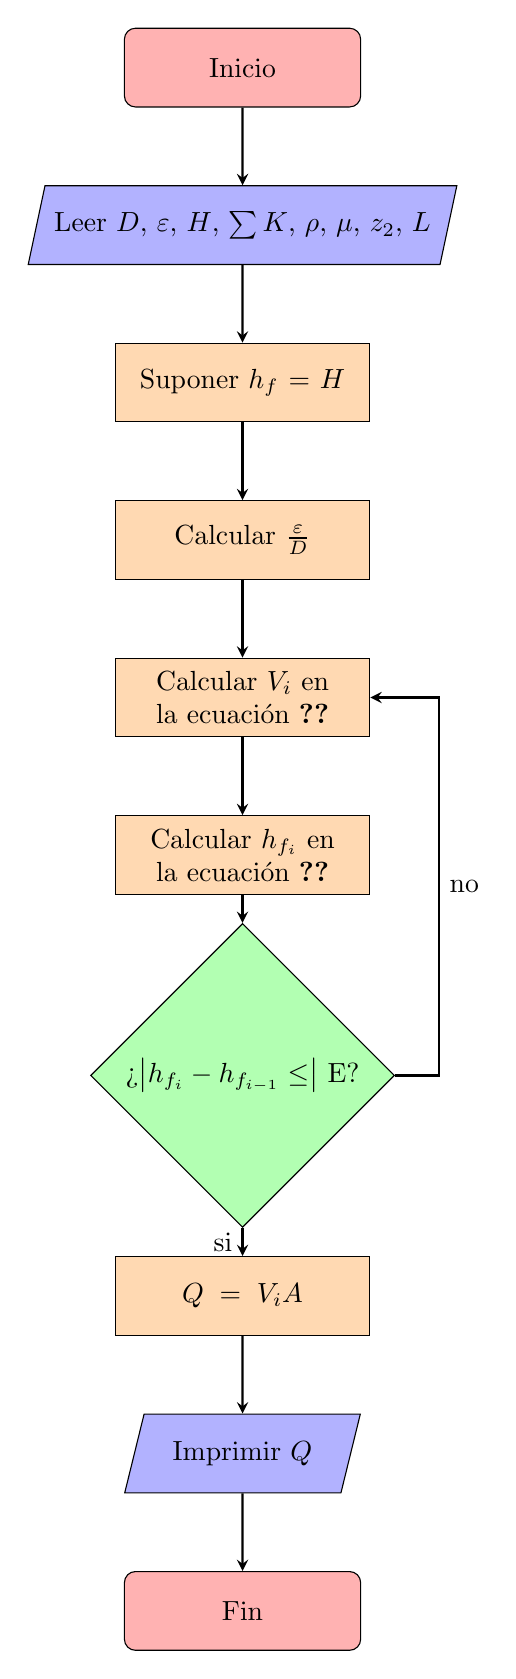
\begin{tikzpicture}[node distance=2cm]

\node (start) [startstop] {Inicio};
\node (in1) [io, below of=start] {Leer $D$, $\varepsilon$, $H$, $\sum K$, $\rho$, $\mu$, $z_2$, $L$};
\node (pro1) [process, below of=in1] {Suponer $h_f = H$};
\node (pro2) [process, below of=pro1] {Calcular $\frac{\varepsilon}{D}$};
\node (pro3) [process, below of=pro2] {Calcular $V_i$ en la ecuaci\'on~\ref{comp8}};
\node (pro4) [process, below of=pro3] {Calcular $h_{f_i}$ en la ecuaci\'on~\ref{com3}};
\node (dec1) [decision, below of=pro4, yshift=-0.8cm] {¿$\left| h_{f_i} - h_{f_{i-1}}\leq \right|$ E?};

%\node (pro2b) [process, right of=dec1, xshift=2cm] {Process 2b};
\node (pro5) [process, below of=dec1, yshift=-0.8cm] {$Q = V_i A$};
\node (out1) [io, below of=pro5] {Imprimir $Q$};
\node (stop) [startstop, below of=out1] {Fin};

\draw [arrow] (start) -- (in1);
\draw [arrow] (in1) -- (pro1);
\draw [arrow] (pro1) -- (pro2);
\draw [arrow] (pro2) -- (pro3);
\draw [arrow] (pro3) -- (pro4);
\draw [arrow] (pro4) -- (dec1);
\draw [arrow] (dec1)   -- ++(2.5,0)  |- (pro3) node[near start, anchor=west] {no};
\draw [arrow] (dec1) -- node[anchor=east] {si} (pro5);
%\draw [arrow] (pro2b) |- (pro1);
\draw [arrow] (pro5) -- (out1);
\draw [arrow] (out1) -- (stop);

\end{tikzpicture}

%\caption{Diagrama de flujo para comprobaci\'on de dise\~no (adaptado de \cite{saldarriaga})}
%\label{dflow1}
%\end{figure}
%
%En la figura~\ref{dflow1} $E$ representa un error que debe ser determinado por el modelador (e.g. 1x10$^{-5}$). Este procedimiento es aplicable a cualquier problema de comprobaci\'on de dise\~no para cualquier sistema de tuber\'ia simple.
%

\subsection{C\'alculo de la potencia requerida}
A continuaci\'on se describe el proceso para solucionar este tipo de problemas que consiste en determinar la cabeza de energ\'ia de la bomba ($h_b$) y su potencia  ($P$).
\begin{enumerate} 
\item Leer la informaci\'on de entrada: $\varepsilon$, $\rho$, $\mu$ o $\nu$, $L$, $D$, $\sum K$, $Q$, $E1$, $E2$, $h_t$ y $\eta$.
\item Calcular la velocidad como $V=Q/A$.
\item Aplicar el procedimiento descrito en la secci\'on~\ref{sec:pf} o en la secci\'on ~\ref{sec:nr} para calcular $f$.
\item Calcular $h_f$ usando la ecuaci\'on~\ref{com2}.
\item Calcular $h_e$ usando la ecuaci\'on~\ref{com3}.
\item Calcular la cabeza de energ\'ia de la bomba ($h_b$) despejandola de la ecuaci\'on~\ref{com1a}.
\item Calcular la potencia $P$ como:

\begin{equation}
P = \frac{\rho Q g h_b}{\eta}
\label{com12a}
\end{equation}
donde $\eta$ es la eficiencia de la bomba.

\item Imprimir $h_b$ y $P$.
\end{enumerate} 

\subsection{Disen\~o de la  tuber\'ia}
A continuaci\'on se describe el proceso para solucionar este tipo de problemas que consiste en determinar el diametro \'optimo comercial de la tuber\'ia.
\begin{enumerate} 
\item Leer la informaci\'on de entrada: $\varepsilon$, $\rho$, $\mu$ o $\nu$, $L$, $D$, $\sum K$, $Q$, $E1$, $E2$, $h_t$ y $\eta$.
\item Asumir un di\'ametro comercial inicial $D_i$ para la tuber\'ia. El $D_i$ inicial debe ser peque\~no (e.g. 1 pulg.) pero no tan peque\~no ya que el procedimiento no converge.
\item \label{fri} Aplicar el procedimiento descrito en la secci\'on~\ref{sec:pf} o en la secci\'on ~\ref{sec:nr}. Note que lo \'unico que cambia dentro de estos procedimientos es que la velocidad $V$ es calculada usando la ecuaci\'on~\ref{com7}; ya no es un dato de entrada. De aqui sale un valor de $f$ y $V$.
\item Calcular el nuevo caudal $Q_n =VA$ usando $D_i$, donde $A=\frac{\pi D_i^2}{4}$.
\item Si $Q_n >= Q $ ir a ~\ref{pri}. Si $Q_n < Q$ tomar el siguiente di\'ametro comercial superior $D_{i+1}$ e ir a ~\ref{fri}.
\item \label{pri} Imprimir $D$.
\end{enumerate} 

El dise\~no \'optimo busca, en la mayoria de los casos, la soluci\'on m\'as econ\'omica. Por lo tanto es necesario muchas veces dise\~nar con otros materiales (diferente valor de $\varepsilon$) para encontrar  la mejor soluci\'on.
 

%%%%%%%%
\section{Sistemas de tuber\'ias en serie} 
Las tuber\'ias en serie son dos o mas tuber\'ias conectadas una tras de otra con diferente di\'ametro o rugosidad (material) o ambos (ver figura~\ref{ttuse}). Estas tuber\'ias son muy comunes en sistemas de riego localizado de alta frequencia o en l\'ineas de coducci\'on para acueductos veredales. Al igual que en la secci\'on~\ref{tubs}, aqu\'i se describir\'an las ecuaciones generales para resolver problemas relacionados con tuber\'ias en serie y se explicar\'an los procedimientos para resolver los tres problemas en tuber\'ias: 1) Comprobaci\'on de dise\~no, 2) c\'alculo de la potencia y 3) dise\~no de las tuber\'ias.

% Fig 5.1 from Salda 
\begin{figure}[h]
\centering
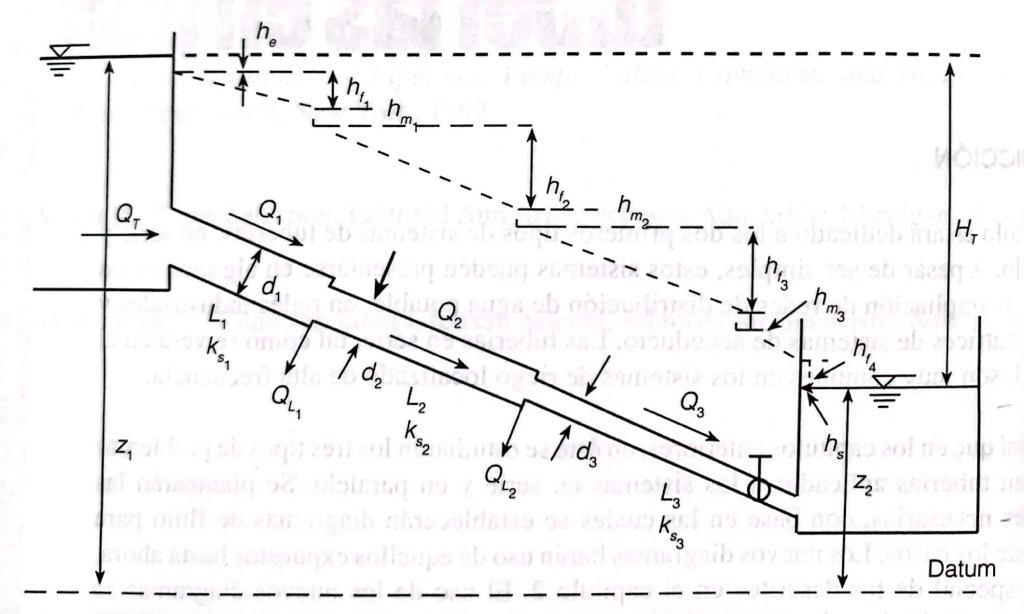
\includegraphics[width=8cm]{comp2.jpeg}
\caption{Tres tuber\'ias en serie conectando dos tanques en donde $Q_{L_i}$ representa un caudal lateral de salida al final de la tuber\'ia $i$ (tomado de \cite{saldarriaga}).} 
\label{ttuse}
\end{figure}

\subsection{Ecuaciones para la soluci\'on de problemas}
Teniendo en cuenta las tuberias en serie de la figura~\ref{ttuse}, se plantean las siguientes ecuaciones:
\begin{itemize}
\item Conservaci\'on de la energ\'ia
\begin{equation}
\Delta E = E1-E2 = H_T = z_1 - z_2 = h_e + h_{f_1} + h_{m_1} + h_{f_2} + h_{m_2} + h_{f_3} + h_{m_3} + h_s
\label{cesp}
\end{equation}
donde $H_T$ es la diferencia de niveles entre los dos tanque; la energ\'ia total disponible en el sistema, $h_e$ p\'erdidas menores de entrada, $h_{f_i}$ p\'erdidas por fricci\'on en el tubo $i$, $h_{m_i}$ p\'erdidas menores (por v\'alvulas, uniones, etc) en la tuber\'ia $i$ y $h_s$ p\'erdidas por salida.

Para un numero $n$ de tuber\'ias en series la ecuaci\'on~\ref{cesp} se puede excribir como:
\begin{equation}
H_T = h_e + \sum_{i=1}^{n} h_{f_i} + \sum_{i=1}^{n} \sum_{j=1}^{m} h_{m_{i,j}} + h_s 
\label{cesp1}
\end{equation}

donde $m$ es numero de accesorios en la tuber\'ia $i$; $m$ puede ser variable. La ecuaci\'on~\ref{cesp1} establece que la energ\'ia disponible en el sistema se disipa en p\'erdidas a lo largo de la tuber\'ia. Puede haber el caso en el cual tengamos, por ejemplo, una tuber\'ia horizontal por lo cual una bomba ser\'ia necesaria para impulsar el flujo por lo que en la parte izquierda de la ecuaci\'on~\ref{cesp} tendr\'iamos $H_T + h_b$. Tambi\'en se puede dar el caso de una turbina en alguna secci\'on de la tuber\'ia por lo que habria que sumarle a la derecha de la ecuaci\'on $h_t$.

Desarrollando la ecuaci\'on~\ref{cesp1}, se tiene:

\begin{equation}
\color{red}\boxed{\color{black} H_T = K_e \left( \frac{V^2}{2g} \right)_1 + \sum_{i=1}^{n} \left( f\frac{L}{D}\frac{V^2}{2g} \right)_i + \sum_{i=1}^{n} \left(\frac{V^2}{2g}\right)_i \sum_{j=1}^{m} K_j + K_s \left( \frac{V^2}{2g} \right)_n }
\label{cesp2}
\end{equation}

\item Conservaci\'on de la masa o ecuaci\'on de continuidad:

\begin{equation}
Q_T = Q_1 = Q_2 + Q_{L_1} = Q_3 + Q_{L_1} + Q_{L_2}
\label{cesp3}
\end{equation}

Donde $Q_i$ es el caudal que viaja por la tuber\'ia $i$ y $Q_{L_i}$ es el caudal derivado de la tuber\'ia $i$. La ecuaci\'on~\ref{cesp3} se puede expresar de forma mas compacta como:

\begin{equation}
\color{red}\boxed{\color{black} Q_T = Q_i + \sum_{j=1}^{i-1} Q_{L_j} }
\label{cesp4}
\end{equation}

En caso de que no existiera derivaciones ($Q_{L_i} = 0$) la ecuaci\'on~\ref{cesp4} queda como:

\begin{equation}
\color{red}\boxed{\color{black} Q_T = Q_1 = ...= Q_i = ...  = Q_n }
\label{cesp5}
\end{equation}

\end{itemize}

\subsection{Comprobaci\'on de dise\~no}
Se desea calcular el valor de $Q_T = Q_1$. Antes de describir el proceso de c\'alculo, deduciremos una ecuaci\'on que se utilizar\'a para resolver este tipo de problemas. 

De la ecuaci\'on de Darcy-Weisbach, despejando el factor de fricci\'on se tiene que:

\begin{equation}
f = \frac{h_f D 2g}{L V^2}
\label{com41}
\end{equation}

Sacando ra\'iz cuadrada e invirtiendo los t\'erminos a ambos lados se tiene:

\begin{equation}
\frac{1}{\sqrt{f}} = \frac{V\sqrt{L}}{\sqrt{h_f D 2g}}
\label{com51}
\end{equation}

Igualando a la ecuaci\'on de Colebrook-White, se tiene:

\begin{equation}
\frac{V\sqrt{L}}{\sqrt{h_f D 2g}}= -2 \log \left( \frac{\varepsilon}{3.7D} + \frac{2.52}{Re \sqrt{f}} \right) 
\label{com71}
\end{equation}

Reemplazando $Re = \frac{VD}{\nu}$ y la ecuaci\'on~\ref{com51} en la ecuaci\'on~\ref{com71} y despejando la velocidad, se tiene:

\begin{equation}
\color{red}\boxed{\color{black} V= \frac{-2\sqrt{2gD h_f}}{\sqrt{L}} \log \left( \frac{\varepsilon}{3.7D} + \frac{2.52 \nu \sqrt{L}}{D \sqrt{2gD h_f}} \right) }
\label{com81}
\end{equation}

Note que la ecuaci\'on~\ref{com81} es explicita para la velocidad $V$. 

A continuaci\'on se describe el proceso para solucionar este tipo de problemas que consiste en determinar $Q_T = Q_1$.

\begin{enumerate}
\item Leer: $\rho$, $\mu$ o $\nu$, $K_e$ (coef. de p\'erdidas a la entrada), $K_s$ (coef. de p\'erdidas a la salida), $E1$ y $E2$. Tambi\'en, para cada tuber\'ia $i$, leer: $L_i$, $D_i$, $\sum K_i$, $Q_{L_i}$, $h_{b_i}$, $h_{t_i}$ y $\eta_i$ (eficiencia de la bomba o turbina). Esta lectura se debe hacer para las $n$ tuber\'ias del sistema.
\item Para llevar a cabo este proceso es necesario, para la primera iteraci\'on, asumir un valor inicial de $h_{f_1} $. Se ha encontrado que $h_f \propto \frac{L}{D^5}$, de acuerdo con esto, \cite{saldarriaga} ha establecido que este valor inicial de $h_{f_1}$ se puede expresar como:

\begin{equation} 
h_{f_1} = E1-E2 = H_T \frac{L_1 / D_1^5}{\sum_{i=1}^{n} L_i / D_i^5 }
\label{cpd1}
\end{equation}

\item \label{vve} Para la tuber\'ia $i=1$: calcular el valor de $V_1$ usando la ecuaci\'on~\ref{com81}, calcular el caudal $Q_T = Q_1 = V_1 A_1$, calcular el valor de $f_1$ usando uno de los dos procedimientos descritos en la secciones~\ref{sec:pf} y ~\ref{sec:nr}, calcular $h_{f_1}$ utilizando la ecuaci\'on~\ref{com2} y $h_{m_1}$  utilizando la ecuaci\'on~\ref{com3}.

\item Para el resto de tuber\'ias  $i = 2 ... n$: calcular el caudal $Q_i$ usando la ecuaci\'on~\ref{cesp4}, calcular la velocidad $V_i = Q_i /A_i$, $f_i$ usando uno de los dos procedimientos descritos en la secciones~\ref{sec:pf} y ~\ref{sec:nr}, calcular $h_{f_i}$ utilizando la ecuaci\'on~\ref{com2} y $h_{m_i}$  utilizando la ecuaci\'on~\ref{com3}.

\item Calcular la p\'erdida de energ\'ia total estimada $\hat{H_T}$ usando la ecuaci\'on~\ref{cesp1}. Si $|\hat{H_T} - H_T | \leq \eta$ donde $\eta$ es un error  (e.g. $\eta$ = 1x10$^{-6}$), ir a ~\ref{prf}. Si $|\hat{H_T} - H_T | > \eta$, actualizar el valor de $h_{f_1}$, como:

\begin{equation} 
h_{f_1}^t  = h_{f_1}^{t-1}  + \Delta h_{f_1}
\label{cpd2}
\end{equation}

donde $\Delta h_{f_1}$, se calcula como

\begin{equation} 
\Delta h_{f_i} = (H_T - \hat{H_T}) \frac{L_1 / D_1^5}{\sum_{i=1}^{n} L_i / D_i^5 }
\label{cpd3}
\end{equation}

Una v\'ez calculado el nuevo $h_{f_1}$ ir a ~\ref{vve}.

\item \label{prf} Imprimir $Q_i$ donde $i = 1 ... n$. 

\end{enumerate}
\subsection{C\'alculo de la potencia requerida}
A continuaci\'on se describe el proceso para solucionar este tipo de problemas que consiste en determinar la cabeza de energ\'ia de la bomba ($h_b$) y su potencia  ($P$).

\begin{enumerate}
\item Leer: $\rho$, $\mu$ o $\nu$, $K_e$ (coef. de p\'erdidas a la entrada), $K_s$ (coef. de p\'erdidas a la salida), $E1$, $E2$ y $Q_T = Q_1$. Tambi\'en, para cada tuber\'ia $i$, leer: $L_i$, $D_i$, $\sum K_i$, $Q_{L_i}$, $h_{t_i}$ y $\eta_i$ (eficiencia de la bomba o turbina). Esta lectura se debe hacer para las $n$ tuber\'ias del sistema.
\item Utilizando la ecuaci\'on~\ref{cesp4}, calcular el valor de $Q_i$ para $i=2...n$.
\item Para cada una de las tuber\'ias $i=1...n$, calcular: la velocidad como $V_i = Q_i /A_i $, $f_i$ usando uno de los dos procedimientos descritos en la secciones~\ref{sec:pf} y ~\ref{sec:nr}, calcular $h_{f_i}$ utilizando la ecuaci\'on~\ref{com2} y $h_{m_i}$  utilizando la ecuaci\'on~\ref{com3}.
\item Calcular la cabeza de energ\'ia de la bomba ($h_b$) despejandola de la ecuaci\'on~\ref{com1a}. Note que  en esta ecuaci\'on, $h_f$ es la sumatoria de todas $h_{f_i}$ y $h_m$ es la sumatoria de todas las $h_{m_i}$. 
\item Calcular la potencia $P$ usando la ecuaci\'on~\ref{com12a}.
\item Imprimir $h_b$ y $P$.
\end{enumerate}



\subsection{Disen\~o de la  tuber\'ia}
Como se habia mencionado anteriormente, el dise\~no, y en este caso, de tuber\'ias en serie es un problema complejo por que eso implica buscar, en la mayoria de los casos, la soluci\'on optima desde el punto de vista economico. Por esto, no solo basta con determinar el diametro si no tambien el material de la tuber\'ia. A esto hay que sumarle que los coeficiente de perdida dependen del material de la tuber\'ia, esta es otra variable que hay que tener en cuenta. Esto quiere decir que pueden existir multiples soluciones para un mismo problema. 

A continuaci\'on se describe el proceso para solucionar este tipo de problemas que consiste en determinar el diametro \'optimo comercial $D_i$ de la tuber\'ia para $i=1...n$. En este proceso se asume que el material es un dato dado. 

\begin{enumerate}
\item Leer: $\rho$, $\mu$ o $\nu$, $K_e$ (coef. de p\'erdidas a la entrada), $K_s$ (coef. de p\'erdidas a la salida), $E1$, $E2$ y $Q_T = Q_1$. Tambi\'en, para cada tuber\'ia $i$, leer: $L_i$,  $\sum K_i$, $Q_{L_i}$, $h_{b_i}$, $h_{t_i}$ y $\eta_i$ (eficiencia de la bomba o turbina). Esta lectura se debe hacer para las $n$ tuber\'ias del sistema.
\item Utilizando la ecuaci\'on~\ref{cesp4}, calcular el valor de $Q_i$ para $i=2...n$.
\item Inicializar $h_{f_i}$ para cada tuber\'ia $i=1...n$. I-pai Wu en 1975 encontr\'o la siguiente ecuaci\'on para inicializar $h_{f_i}$ antes de iniciar las iteraciones:
\begin{equation} 
h_{f_i} = H_T \frac{L_i \cos \theta_i}{\sum_{i=1}^n L_i \cos \theta_i}
\label{desp1}
\end{equation}
donde $\theta_i$ es el angulo formado entre la horizontal y la tuber\'ia. Usualmente este angulo es el mismo para todas las tuber\'ias ya que todas tienen la misma pendiente, por lo tanto $\theta = \frac{z_1 - z_2}/\sum_{i=1}^n L_i$, donde $z_1$ es la altura a la entrada del sistema y $z_2$ es la altura a la salida del sistema.
\item \label{fff} Para cada tuber\'ia $i=1...n$
\begin{enumerate}
\item \label{fri} Asumir un di\'ametro comercial inicial $D_i$. El $D_i$ inicial debe ser peque\~no (e.g. 1 pulg.) pero no tan peque\~no ya que el procedimiento no converge.
\item Aplicar el procedimiento descrito en la secci\'on~\ref{sec:pf} o en la secci\'on ~\ref{sec:nr}. Note que lo \'unico que cambia dentro de estos procedimientos es que la velocidad $V$ es calculada usando la ecuaci\'on~\ref{com7}; ya no es un dato de entrada. De aqui sale un valor de $f$ y $V$.
\item Calcular el nuevo caudal $Q_{n_i} =V_i A_i $ usando $D_i$, donde $A_i =\frac{\pi D_i^2}{4}$.
\item Si $Q_{n_i} >= Q_i $ ir a ~\ref{pri}. Si $Q_{n_i} < Q_i $ tomar el siguiente di\'ametro comercial superior $D_{i+1}$ e ir a ~\ref{fri}.
\end{enumerate}
\item \label{pri} Para cada tuber\'ia $i=1...n$, calcular la velocidad real como $V_{R_i} = Q_i / A_i$
\item Para cada tuber\'ia $i=1...n$, y con el $D_i$ y $V_{R_i}$, calcular $f_i$ usando el procedimiento descrito en la secci\'on~\ref{sec:pf} o en la secci\'on ~\ref{sec:nr}.
\item Para cada tuber\'ia $i=1...n$, calcular $h_{f_{Ri}}$ utilizando la ecuaci\'on~\ref{com2} y $h_{m_{Ri}}$  utilizando la ecuaci\'on~\ref{com3}. Usar en estas ecuaciones $D_i$ y $V_{R_i}$.
\item La energ\'ia del sistema a la salida de la tuber\'ia $n$ suele ser superior a la energ\'ia requerida del sistema all\'i ($E2$), por lo que usualmente se utiliza una valvula para hacer caer la energ\'ia a $E2$. Dicha caida $h_{m_v}$, se calcula como:
\begin{equation} 
h_{m_v} = H_T - \sum_{i=1}^n h_{f_{Ri}} - \sum_{i=1}^n h_{m_{Ri}}
\label{desp2}
\end{equation}
\item Si $h_{m_v} > 0$ y $h_{m_v} \approx E2$, ir a ~\ref{ttt}. Si $h_{m_v} >> E2$, para cada tuber\'ia $i=1...n$, actualizar el valor de $h_{f_i}$ para la siguiente iteraci\'on como:
\begin{equation} 
h_{f_i} = h_{f_{Ri}} + h_{m_v}
\label{desp3}
\end{equation}
Luego ir a ~\ref{fff}.

\item \label{ttt} Imprimir $D_i$ para $i=1...n$.

\end{enumerate}

Es importante revisar que $h_{m_v}$ sea positivo, de lo contrario esto supondr\'ia presiones negativas que podrian generar cavitaci\'on en el sistema. El procedimiento anterior puede ser repetido para diferentes materiales de tuber\'ia (diferentes valores de $\varepsilon$) con el fin de escoger el dise\~no m\'as econ\'omico.


%%%%%%%
\section{Sistemas de tuber\'ias en paralelo} 

%%%%%%%%
\section{Sistemas de tuber\'ias ramificadas} 

%%%%%%%%
\section{Redes de distribuci\'on: M\'etodo de an\'alisis de Cross}

%%%%%%%%
\section{Redes de distribuci\'on: M\'etodo de an\'alisis lineal}




% REFERENCES
\bibliographystyle{plain} % We choose the "plain" reference style
\bibliography{refs} % Entries are in the refs.bib file



\end{document}
